\documentclass[11pt]{article}

\usepackage{custom}

\title{Compte-Rendu TP C++ \#1}
\author{{\sc Renault} Benoit, {\sc Espeute} Clément}
\date{14 septembre 2015}

\usepackage{listings}
\usepackage{graphicx}

\definecolor{commentColor}{rgb}{0.7,0.7,0.7}
\definecolor{mygray}{rgb}{0.5,0.5,0.5}
\definecolor{mymauve}{rgb}{0.58,0,0.82}
\lstset{language=bash} 
\lstset{ %
  backgroundcolor=\color{black!5},   % choose the background color; you must add \usepackage{color} or \usepackage{xcolor}
  basicstyle=\footnotesize\ttfamily,        % the size of the fonts that are used for the code
  breakatwhitespace=false,         % sets if automatic breaks should only happen at whitespace
  breaklines=true,                 % sets automatic line breaking
  captionpos=b,                    % sets the caption-position to bottom
  commentstyle=\color{commentColor},    % comment style
  deletekeywords={...},            % if you want to delete keywords from the given language
  escapeinside={\%*}{*)},          % if you want to add LaTeX within your code
  extendedchars=true,              % lets you use non-ASCII characters; for 8-bits encodings only, does not work with UTF-8
  frame=single,	                   % adds a frame around the code
  keepspaces=true,                 % keeps spaces in text, useful for keeping indentation of code (possibly needs columns=flexible)
  keywordstyle=\color{blue},       % keyword style
  language=C++,                 % the language of the code
  otherkeywords={*,...},            % if you want to add more keywords to the set
  numbers=left,                    % where to put the line-numbers; possible values are (none, left, right)
  numbersep=5pt,                   % how far the line-numbers are from the code
  numberstyle=\tiny\color{mygray}, % the style that is used for the line-numbers
  rulecolor=\color{black!20},         % if not set, the frame-color may be changed on line-breaks within not-black text (e.g. comments (green here))
  showspaces=false,                % show spaces everywhere adding particular underscores; it overrides 'showstringspaces'
  showstringspaces=false,          % underline spaces within strings only
  showtabs=false,                  % show tabs within strings adding particular underscores
  stepnumber=1,                    % the step between two line-numbers. If it's 1, each line will be numbered
  stringstyle=\color{mymauve},     % string literal style
  tabsize=2,	                   % sets default tabsize to 2 spaces
  title=\lstname,                   % show the filename of files included with \lstinputlisting; also try caption instead of title
  postbreak=\raisebox{0ex}[0ex][0ex]{\tt\color{red}-> }
}


\begin{document}
\pagestyle{fancy}
\maketitle

\section[Spécifications]{Spécifications de la classe <Collection>}

\subsection{Présentation générale}
<Collection> a pour rôle de gérer le stockage, la modification et l'affichage d'un ensemble de \emph{nombres entiers}. Le stockage est réalisé dans un tableau d'entiers (int) géré de façon dynamique simple, c'est à dire que l'on a également deux attributs de type entier non-signé, l'un servant à connaître le nombre d'éléments actuellement présents dans le tableau, l'autre servant à connaître la taille allouée au tableau. Le cahier des charges ne l'exigeant pas, les redondances sont acceptées et les valeurs ne sont pas triées.

\subsection{Présentation des méthodes}

\subsubsection*{Constructeur n°1}
Créé une collection pouvant accueillir un nombre entier non-signé donné d'éléments sans avoir besoin d'être redimensionnée, et alloue la mémoire nécessaire au tableau.

\subsubsection*{Constructeur n°2}
Créé une collection pouvant accueillir un nombre entier non-signé donné d'éléments sans avoir besoin d'être redimensionnée, et alloue la mémoire nécessaire au tableau. Les valeurs du tableau d'entiers quelconque dont le pointeur est passé en paramètre sont ensuite ajoutées à la collection (part du contrat : il est à la charge de l’utilisateur de donner une taille égale à celle du tableau passé).

\subsubsection*{Méthode Afficher}
Imprime sur la sortie standard les éléments de la collection dans l'ordre d’apparition du tableau, avec un retour chariot entre chaque élément sur la sortie standard. Si en mode de déboguage, affiche en plus le nombre d’éléments et la taille allouée à la fin de l’affichage des éléments.

\subsubsection*{Méthode Ajouter}
Ajoute la valeur entière donnée dans un élément inséré à l'extrêmité du tableau et fait appel à la fonction d'ajustement si l'insertion implique un dépassement de la taille actuellement allouée au tableau.
\footnote{Tout ajout ou suppression du nombre d'éléments contenus dans le tableau implique bien sûr une mise à jour de l'attribut associé.}

\subsubsection*{Méthode Retirer}
Supprime un nombre entier d'occurences donné d'une valeur entière donnée. Si le nombre d'occurences à retirer donné est négatif, on supprime toutes les occurrences de la valeur entière donnée. La taille du tableau est ajustée après l'opération. 

\subsubsection*{Méthode Ajuster}
Modifie la taille allouee au tableau et le réalloue dynamiquement à une valeur entière non-signée donnée en paramètre. Le redimensionnement est refusé si la taille demandée est inférieur au nombre actuel d'éléments et renvoie un code de retour \texttt{ERR\_TAILLE}.
    
\subsubsection*{Méthode Reunir}
Ajoute les éléments de la collection donnée après ceux de la courante en réajustant la taille allouee du tableau de la courante si celle-ci n'est actuellement pas assez grande pour les accueillir.

\subsubsection*{Méthode Destructeur}

\noindent Effets : Désallocation du tableau.
Détruit la collection courante et libère la mémoire allouée au tableau associé.
\newpage


\section{Les tests}

Afin de vérifier que chaque méthode  notre classe fonctionne, on réalise des tests unitaires sur chacune d'entre elles. La méthode Afficher à été modifiée pour pouvoir donner la taille allouée du tableau et le nombre d'éléments a l'intérieur de celui-ci. Cet affichage peut être désactivé en enlevant le mot clef \texttt{\#define DEBUG} à l'intérieur de \texttt{Collection.h}.

Par ailleurs, afin de rendre les tests plus lisibles dans la console, les textes indiquant les différentes étapes des tests sont imprimés en gras. Si la console ne supporte pas les caractères d'échappement permettant la mise en forme des textes affichés, ils peuvent être désactivé en retirant le mot clef \texttt{\#define~BOLD\_USAGE} à l'interieur de \texttt{main.h}.

\begin{figure}[htp]
\centering
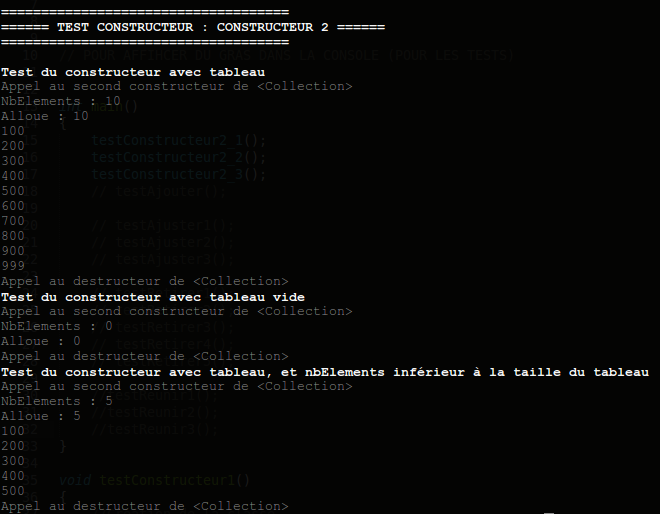
\includegraphics[scale=0.60]{TestConstructeurs.png}
\caption{Exemple des tests pour le second constructeur}
\label{testConstructeur}
\end{figure}

\subsection{Tests pour le deuxième constructeur}

\texttt{testConstructeur2\_X()} sont les méthodes qui effectuent le test pour le second constructeur. 
\begin{description}
	\item[\texttt{testConstructeur2\_1()}] Teste le cas de base où l'on passe un tableau rempli arbitrairement en paramètre du constructeur de la Collection (ainsi que sa taille).
	
	Résultat attendu : La Collection est bien initialisée et elle contient tous les éléments du tableau, et a la même taille. ({\tt allouée = nbElements})
	
	\item[\texttt{testConstructeur2\_2()}] Teste le cas où l'on donne en paramètre un tableau vide.
	
	Résultat attendu : La Collection est bien initialisée et elle est vide. \texttt{allouee} et \texttt{nbElements} est de 0. 
	
	\item[\texttt{testConstructeur2\_3()}] Teste le cas où l'on appelle le constructeur avec en paramètre un tableau et une taille $n$ plus petite que celle du tableau. ({\tt allouée = nbElements =} $n$)
	
	Résultat attendu : La Collection est bien initialisée, et elle est remplie avec les $n$ premiers éléments du tableau passé en paramètre.
\end{description}

\subsection{Tests pour \tt Ajouter}
Le test pour la méthode ajouter comporte 2 tests :

\begin{description}

	\item[\texttt{testAjouter1()}] Ajoute simplement un élément dans la Collection vide avec une taille initiale de 10 (donc pas de redimensionnement nécessaire). On affiche l'état du tableau avant et après l'ajout.
	
	Résultat attendu : Le tableau ne comporte que l'élément ajouté. \texttt{nbElement} vaut 1 et \texttt{alouee} vaut toujours 10. 
	
	\item[\texttt{testAjouter2()}] Ajoute 20 éléments dans une Collection initialement vide. (Donc redimensionnement nécessaire).
	
	Résultat attendu : Le tableau est rempli avec les 20 éléments dans l'ordre dans lequel ils ont été insérés. \texttt{alouee = nbElement = 20}.
	
\end{description}

\subsection{Tests pour Retirer}	
Pour tester la méthode retirer, on remplit au préalable la Collection d'un tableau arbitraire, puis on tente de retirer des éléments. On affiche à chaque fois la Collection avant et après l'opération.

On à alors :
\begin{description}
	\item[\texttt{testRetirer1()}] Retire un élément d'une valeur donnée de la collection.
	
	Résultat attendu : L'élément est supprimé et la collections à bien été redimensionnée à la taille initiale - 1.
	
	\item[\texttt{testRetirer2()}] Retire $n$ éléments d'une valeur donnée de la collection.
	
	Résultat attendu : L'élément est supprimé et la collections à bien été redimensionnée à la taille initiale - $n$.
	
	\item[\texttt{testRetirer3()}] Retire tous les éléments d'une valeur donnée du tableau.
	
	Résultat attendu : Tout les éléments de la valeur donnée sont supprimés et la collections à bien été redimensionnée correctement.
	
	\item[\texttt{testRetirer4()}] Tente de retirer une valeur non présente dans le tableau.
	
	Résultat attendu : Le tableau ne change pas, et il n'y pas d'erreur produite.
	
	\item[\texttt{testRetirer5()}] Retire procéduralement touts les éléments du tableau.
	
	Résultat attendu : Le tableau est vide, \texttt{nbElement = alouee = 0}
\end{description}

\subsection{Tests pour Réunir}
Pour vérifier le bon fonctionnement de la méthode \texttt{Reunir}, on procède à 3 test différents. On affiche à chaque fois les Collections initiales et la Collection correspondant à la réunion des deux.

\begin{description}
	\item[\texttt{testReunir1()}] Crée 2 Collections vides et les réunit.
	
	Résultat Attendu : Aucune différence entre la première collection et la collection réunie.
	
	\item[\texttt{testReunir2()}] Crée 2 Collections et les réunit. Les Collections sont telles que la réunion n'implique pas de redimensionement de la première collection.
	
	Résultat Attendu : La collection réunie contient les éléments de la première suivie des éléments de la seconde. Sa taille \texttt{alouee} est égale à celle de la première collection car il n'y a pas eu de redimensionement.
	
	\item[\texttt{testReunir3()}] Crée 2 Collections et les réunit. La première collection est remplie ce qui implique qu'un redimensionement sera nécessaire lors de la réunion des Collections.
	
	Résultat Attendu : La collection réunie contient les éléments de la première suivie des éléments de la seconde. Sa taille \texttt{alouee} est égale à \texttt{nbElement}
 
\end{description} 

\end{document}